% !TEX program = xelatex
\documentclass{ctexart}
\usepackage{xcolor} % 在latex中使用颜色
\usepackage{booktabs,tabularx,multicol} % 制作表格
\usepackage{tikz,tikz-network}
\usepackage{framed} % 制作文本框
\usepackage{amsmath,amsthm,amssymb,amsfonts}    % 数学符号与字体
\usepackage{hyperref}   % 添加超链接
\usepackage[left=2.0cm, right=2.0cm, top=2.5cm, bottom=2.5cm]{geometry} % 调整页边距
\usepackage{appendix}   % 附录环境
\usepackage{subfig,graphicx}    % 插入照片
\usepackage{float}      % 固定浮动体
\usepackage{lipsum,zhlipsum} %生成一些测试文本
%---------------优雅的插入MATLAB代码---------%
\usepackage{listings,matlab-prettifier} % MATLAB 美化包
\lstset{
        style=Matlab-editor,
        numbers      = left,
        numbersep    = 5pt,
        numberstyle  = \small\color{red},
        frame        = single,
        keepspaces   = true,
        tabsize      = 4,
}
%-------------标题-------------%
\title{BP神经网络在mnist数据集中的应用}
\date{\today}
\author{张阳}

%-----------做一些设置-----------%
\numberwithin{equation}{section}    % 公式标号与section的编号挂钩
\punctstyle{kaiming}    % 调整标点符号大小

%------------自定义一些命令------------%
\newcommand{\upcite}[1]{\textsuperscript{\textsuperscript{\cite{#1}}}}
\newcommand*{\dif}{\mathop{}\!\mathrm{d}}
\def\degree{{}^{\circ}}


%-------------可控列宽的表格--------%
\newcolumntype{L}[1]{>{\raggedright\arraybackslash}p{#1}}
\newcolumntype{C}[1]{>{\centering\arraybackslash}p{#1}}
\newcolumntype{R}[1]{>{\raggedleft\arraybackslash}p{#1}}

%-----------搞个背景-------------%
\usepackage{background}
\backgroundsetup{scale=2, angle=0, opacity = 0.5,contents = {\includegraphics[width=\paperwidth, height=\paperwidth, keepaspectratio]{fig/背景.jpg}}}
%------------- 使得矩阵的最大大小超过 10 x 10-----------------%

%---------------高亮--------------%
\usepackage{soul}
\addtocounter{MaxMatrixCols}{10}
\begin{document}
\maketitle
\begin{abstract}
    本文首先介绍了神经网络的基本知识,重点说明了感知器和S神经元;随后给出了一种求解神经网络的方法:反向传播算法,并给出了数学上的证明。完成准备工作后,将算法应用到了minst手写数学数据集中。为了进一步提升运算速度和改善识别结果,使用了SGD方法,最终数字识别正确率达到了95\%以上。在文章的最后,说明了神经网络的难以训练性。
\end{abstract}
\tableofcontents
\newpage
\section{引言}
近年来,机器学习方兴未艾。2016年,alphago 击败李世石,宣告着围棋这一古老的人类运动人类已经彻底败给了计算机,再一次掀起了广大民众对机器学习的讨论。导航,社交媒体平台,图像识别,情感分析,机器学习的强大效力一次又一次地刷新着我们的认知。在一边赞叹机器学习强大的同时,也有越来越多的学者参与到了它的建设之中,可以说,机器学习就是现在科学界最热门,最激动人心的方向。

神经网络是一种用计算机模拟人脑思维过程的算法,属于机器学习的一种。神经网络的功能很多,在此文中,我们特别以 mnist 数据集为例来制作一个字体识别的神经网络。
\section{生成一个神经网络}
\subsection{神经网络结构}
在人类的大脑中,有着数不清的神经元进行着复杂的化学反应,突触起到了神经元之间的连接作用。这些神经元和突触错综复杂地结合在一起,赋予了我们思考的能力。

受制于硬件水平,我们的神经网络无法达到人类大脑的复杂度,不过好在,我们也不需要让神经网络来承担一个人的所有工作,我们只需要它能够完成一些特殊的任务就好了。

首先,神经网络应当由一些神经元来接受信息,这些神经元构成输入层(input layer);需要一些神经元来运算,处理信息,这些神经元构成隐藏层(hidden layer);还有一些神经元来输出信息,构成输出层(output layer)。神经元当然不能独立工作,因此,我们需要将神经元连接起来,为了简化复杂度,我们认为同层之间的神经元不会由之间的影响,只有非同层的神经元才会互相影响。

于是我们可以简单画一个神经网络来做例子:
\begin{figure}[h]
\centering
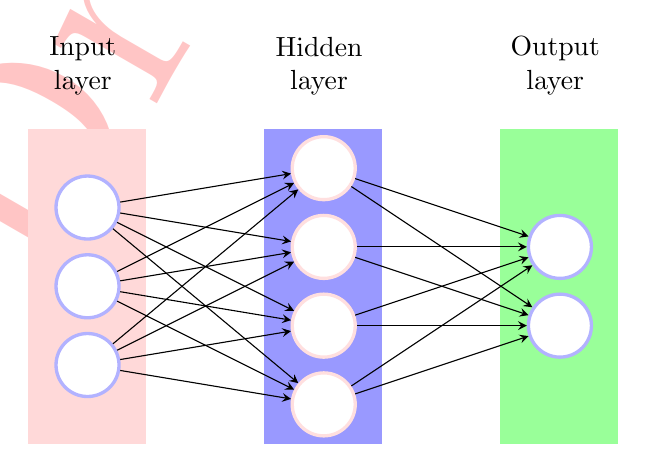
\begin{tikzpicture}
    % 结点样式名称/.style={形状,draw=颜色!色度,fill=填充色!色度,清晰度,minimum size=结点大小}
    [L1Node/.style={circle,draw=blue!30, fill=white!10, very thick, minimum size=8mm},
    L2Node/.style={circle,draw=pink!50, fill=white!10, very thick, minimum size=8mm}]
    
    % 添加背景色,粉色、蓝色和绿色
    % \fill[颜色!透明度]坐标从(0,0)到(15mm,40mm)的矩形node(编号){}
    \fill[pink!60](0,0)rectangle(15mm,40mm)node(b1){};
    % \fill[颜色!透明度]坐标从(30mm,0)到(45mm,40mm)的矩形
    \fill[blue!40](30mm,0)rectangle(45mm,40mm)node(b1){};
    % \fill[颜色!透明度]坐标从(60mm,0)到(75mm,40mm)的矩形
    \fill[green!40](60mm,0)rectangle(75mm,40mm)node(b1){};
    
    % 添加输入层结点
    % \foreach循环\x依次等于1,2,3
    % \node[结点样式] (结点名称) at (结点坐标) {节点内容}
    \foreach \x in {1,...,3}
    \node[L1Node] (a_\x) at (0.76, \x){};		
    
    % 添加隐藏层结点
    \foreach \x in {4,...,7}
    \node[L2Node] (b_\x) at (3.76, \x-3.5){};	
    
    % 添加输出结点
    \foreach \x in {8,9}
    \node[L1Node] (c_\x) at (6.76, \x-6.5){};
    
    % 输入层到隐藏层之间的连线
    \foreach \x in {1,2,3}   % 双层for循环
    {\foreach \z in {4,5,6,7}
        % \draw[线的样式:-{stealth[sep=1pt]}为带箭头的线,[sep箭头距离]
        \draw[-stealth](a_\x)--(b_\z);	
    }
    
    % 隐藏层到输出层之间的连线
    \foreach \z in{4,5,6,7}
    {\foreach \y in{8,9}
        \draw[-stealth](b_\z)--(c_\y);	
    }

    % 添加说明文字
    % 名称node[居中] at (坐标) {结点内容}
    \node[align=center] at (0.7,4.8) {Input\\layer};
    \node[align=center] at (3.7,4.8) {Hidden\\layer};
    \node[align=center] at (6.7,4.8) {Output\\layer};
    
\end{tikzpicture}
\end{figure}
\subsection{神经网络运算方法}
首先,我们先介绍感知器:

一个感知器会接受几个二进制输入,$x_1,x_2,\cdots,x_n$,并产生一个二进制输出。具体来说就是
\begin{equation}
    \label{eqa:1}
    f(x_1,x_2,\cdots,x_n)=\left\{\begin{array}{ll}
        0 & \text { if } \sum_{j} w_{j} x_{j} \leq \text { threshold } \\
        1 & \text { if } \sum_{j} w_{j} x_{j}>\text { threshold }
        \end{array}\right.
\end{equation}

其中,$w_i$ 表示权重。直观上理解,如果感知器受到的刺激超过了某一个预设的阈值,就输出 1;小于这个阈值,就输出 0。

为了简化表达式,我们把 \eqref{eqa:1} 式写成向量的形式。\footnote{$\mathbf{w}$ 和 $b$ 是这个神经元的内在属性,因此自变量只有 $\mathbf{x}$}

\begin{equation}
    f(\mathbf{x})=\left\{\begin{array}{ll}
        0 & \text { if } \mathbf{x}\cdot \mathbf{w}+b<0 \\
        1 & \text { if } \mathbf{x}\cdot \mathbf{w}+b>0
        \end{array}\right.
\end{equation}

其中 $\mathbf{x}=(x_1,x_2,\cdots,x_n),\mathbf{w}=(w_1,w_2,\cdots,x_n),\mathbf{x}\cdot\mathbf{w}=\sum x_iw_i$, $b$ 为预设的阈值。

如果令 $z=\mathbf{x}\cdot\mathbf{w}$,上式可以进一步化简为:

\begin{equation}
    f(\mathbf{x})=\left\{\begin{array}{ll}
        0 & \text { if } z<0 \\
        1 & \text { if } z>0
        \end{array}\right.
\end{equation}

\begin{figure}[htp]
    \centering
    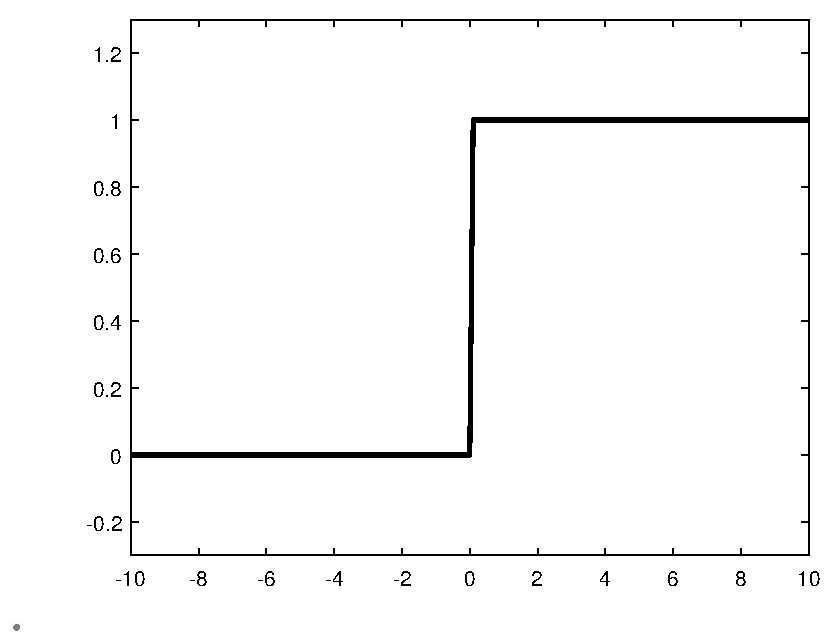
\includegraphics[width=0.7\linewidth]{fig/感知器}
    \caption{感知器}
    \label{fig:}
\end{figure}

可以直观地看到,在 $z=0$ 初函数值发生了突变,这就意味着函数无法在该点处求导,不具有良好的分析性质,为此,我们引入 S 神经元

\begin{equation}
    f(\mathbf{x})= \frac{1}{1+\exp(-z)}
\end{equation}

\begin{figure}[htp]
    \centering
    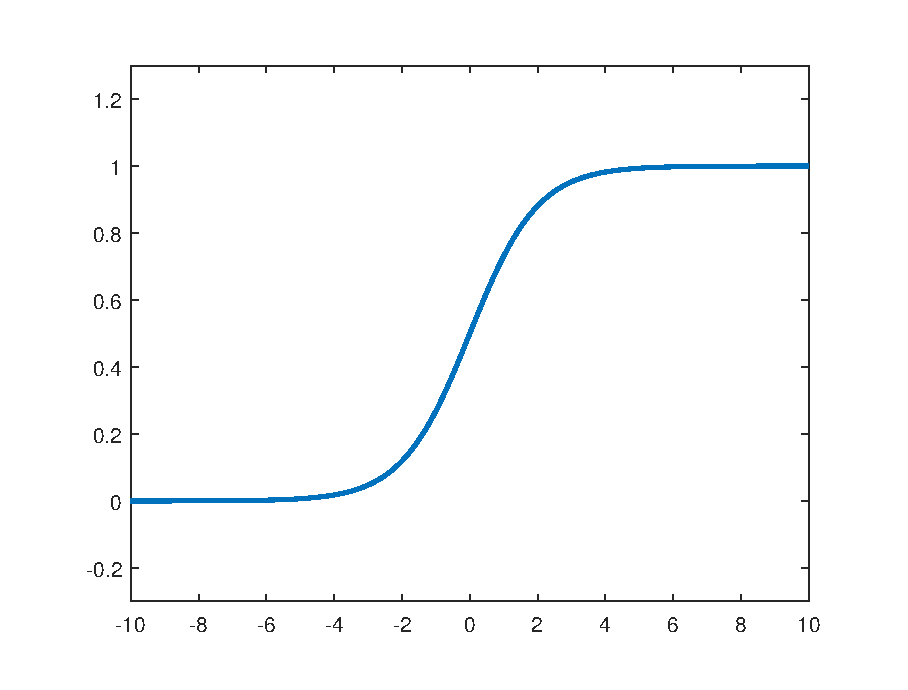
\includegraphics[width=0.7\linewidth]{fig/S神经元}
    \caption{S神经元}
\end{figure}

可以看到,当 $z$ 的值较大的时候,$f(\mathbf{x})\approx1$,当 $z$ 的值较小的时候,$f(\mathbf{x})\approx0$,这与我们前面提出的感知器是一样的。而当 $ z $ 在零附近的时候,$f(\mathbf{x})$ 平滑地从 $0$ 过渡到 $1$。由此,我们可以得出:S 神经元可以胜任感知器的大部分工作,并且具有良好的分析性质我们可以不妨选用这样一个 S 神经元作为感知器。

重新回到我们的神经网络,输入层的神经元仅用作读取数据和传递数据,不参与运算。而隐藏层的每一个神经元都要接收来自上一层的所有 $x_i$ 并向下一层输出 $f(\mathbf{x})$。输出层的神经元也要接受来自上一层所有 $x_i$,并给出一个输出结果,结合所有输出层的神经元的输出结果,我们就可以得到该神经网络的输出结果。
% \begin{figure}[h]
%     \centering
% \begin{tikzpicture}
%     \Vertex[label=$x_1$,]{A1}
%     \Vertex[label=$x_2$,y=-1]{A2}
%     \Vertex[label=$x_3$,y=-2]{A3}
%     \Vertex[label=感知器,x = 2,y=-1,size=1]{B}
%     \Vertex[label=y,fontsize=\large,x=5,y=-1,style={opacity =0}]{C}
%     \Edge[Direct=true](A1)(B)
%     \Edge[Direct=true](A2)(B)
%     \Edge[Direct=true](A3)(B)
%     \Edge[Direct=true](B)(C)
%     \end{tikzpicture}
% \end{figure}

\subsection{本例中的神经网络}
\begin{figure}[htp]
    \centering
    
\includegraphics[width=0.7\linewidth]{fig/图片.eps}
    \caption{minst数据集示意图}
\end{figure}

\label{subsec:神经网络}
MNIST 数据集包含了6万张手写数字图片的训练集,和1万的测试集,每张规格为 $28\times28$ 大小的灰度图像\footnote{在电子计算机领域中,灰度(Gray scale)数字图像是每个像素只有一个采样颜色的图像。这类图像通常显示为从最暗黑色到最亮的白色的灰度,尽管理论上这个采样可以是任何颜色的不同深浅,甚至可以是不同亮度上的不同颜色。灰度图像与黑白图像不同,在计算机图像领域中黑白图像只有黑白两种颜色,灰度图像在黑色与白色之间还有许多级的颜色深度。}。经过简单的数据处理,可以将图片转变为一个 $784\times 1$ 的矩阵,即将原 $28\times28$ 按列排列;将标签转变为 $10\times 1$ 的向量,如果标签为 $i$ ,则除第 $i+1$ 个元素为一外,其余所有元素都为零,例如:$[0,0,0,0,1,0,0,0,0,0]$ 表示这个图片的标签为 $4$。

基于此,输入层我们设计为 $28\times28=784$ 个神经元,输出层为 10 个神经元。而中间层,这里我们设计成由 30 个神经元构成的只有一层的隐藏层,当然,我们这里也可以改成 50 个或者 10 个神经元,都没有太大的问题,但这会对后面的运算速度和结果产生些许的影响。

神经网络最终的输出结果要根据输出层的神经元的输出来判断,判断依据是,如果第 $i$ 个神经元的输出值最大(后面我们会知道,这实际上是最接近于1),那么我们就认为这个图像对应的数字是 $i$。

至于 $b$\footnote{可以看出,在 S 神经元中,b 不再代表感知器中那个突变的阈值,因此将其改名为偏置以作区别},$w$,这里我们采用随机生成的方式。具体来说,采用标准正态分布。

这样,我们就设计了一个三层的神经网络,第一层有 784 个神经元,第二层有 30 个神经元,第三层有 10 个神经元,初始参数均由标准正态分布随机数生成。
\section{bp神经网络的学习过程}
让我们回想我们作为人类是如何学习认识数字的,当我们第一次接触数字的时候,我们也并不能说出它代表数字几,但我们在他人的帮助下,在一次次的失败中获得了经验,从而具有了判断能力。

神经网络也是一样,不难看出,对于一张确定的照片,影响输出结果的就是 权重 $\omega$ 和偏置 $b$。于是我们下一步的方向就是,当神经网络犯错的时候,也就是做了错误分类的时候,如何引导神经网络选择正确的权重 $\omega$ 和偏置 $b$,从而纠正错误。

这样的学习方法有很多,在微积分中我们学到,函数值沿梯度的反方向下降速度最快,这里我们采用同样的思路。这引入了两个个新问题,如何定义函数,以及如何对函数求导。

为方便后面公式推导,这里给出符号说明:
\begin{table}[h]
    \centering
    \begin{tabular}{cc}
        \toprule
        符号 & 符号含义\\
        \midrule
        $a^l$ & 第 $l$ 层的激活值(输出值)矩阵\\
        $b^l$ & 第 $l$ 层的偏置矩阵\\
        $w^l$ & 第 $l$ 层的权重矩阵\\
        $a_j^l$ & 第 $l$ 层第 $j$ 个神经元的激活值(输出值)\\
        $b_j^l$ & 第 $l$ 层第 $j$ 个神经元的偏置\\
        $w^l_{jk}$ & 连接第 $l-1$ 层的第 $k$ 个神经元到第 $l$ 层的第 $j$ 个神经元的权重\\
        $\odot$ & Hadamard 乘积 $(s \odot t)_{j}=s_{j} t_{j}$\\
        $\sigma(x)$ & $\frac{1}{1+\exp(-x)}$\\
        \bottomrule
    \end{tabular}
\end{table}
\subsection{损失函数}
损失函数是用于计算误差,评价模型预测结果是否准确的一个函数。因此,当模型的输出值与真实值非常接近的时候,损失函数应当接近零。为了便于后面求导,以及形式的简洁性,我们采用二次代价函数:

\begin{equation}
    C=\frac{1}{2n}\sum_{n}\lvert\lvert y(x)-a^L(x)\rvert\rvert^2_2
\end{equation}

其中 $n$ 是训练样本的总数;求和运算遍历了每个训练样本 $x$;$y = y(x)$ 是对应的正确的⽬标输出;$L$ 表⽰⽹络的层数;$a^L = a^L(x)$ 是当输⼊是 $x$ 时的⽹络输出的激活值向量。

特别的,我们设 
\begin{equation}
    C_x=\frac{1}{2}\lvert\lvert y(x)-a^L(x)\rvert\rvert^2_2
\end{equation}
表示对于取定的一个输入值 $x$ 的损失函数。
\subsection{反向传播算法}
我们定义 $l$ 层的第 $j$ 个神经元上的误差 $\delta^l_j$ 为

\begin{equation}
    \delta_j^l=\frac{\partial C}{\partial z_j^l}
\end{equation}

利用 $\delta$ 我们可以用下面的方程计算 $\frac{\partial C}{\partial b_{j}^{l}}$,$\frac{\partial C}{\partial w_{j k}^{l}}$

\begin{subequations}
    \label{eqa:2}
    \begin{align}
    & \delta^{L}=\nabla_{a} C \odot \sigma^{\prime}\left(z^{L}\right) \label{eqa:2-1}\\
    & \delta^{l}=\left(\left(w^{l+1}\right)^{T} \delta^{l+1}\right) \odot \sigma^{\prime}\left(z^{l}\right) \label{eqa:2-2}\\
    & \frac{\partial C}{\partial b_{j}^{l}}=\delta_{j}^{l} \label{eqa:2-3}\\
    & \frac{\partial C}{\partial w_{j k}^{l}}=a_{k}^{l-1} \delta_{j}^{l} \label{eqa:2-4}
    \end{align}
\end{subequations}

下面给出上式的证明过程。

对于 \eqref{eqa:2-1} 式:
\begin{proof}
    \begin{equation}
        \begin{aligned}
            \delta_j^L&=\frac{\partial C}{\partial z_j^L}\\
            &=\frac{\partial C}{\partial a_k^j}\frac{\partial a_k^j}{\partial z_j^L}\\
            &=\frac{\partial C}{\partial a_k^j}\sigma'(z^L)
        \end{aligned}
    \end{equation}
    这就是 \eqref{eqa:2-1} 式的分量形式
\end{proof}

对于 \eqref{eqa:2-2} 式:
\begin{proof}
    \begin{equation}
        \begin{aligned}
            \delta_{j}^{l} &=\frac{\partial C}{\partial z_{j}^{l}} \\
            &=\sum_{k} \frac{\partial C}{\partial z_{k}^{l+1}} \frac{\partial z_{k}^{l+1}}{\partial z_{j}^{l}} \\
            &=\sum_{k} \frac{\sum_{j} w_{k j}^{l+1} \sigma\left(z_{j}^{l}\right)+b_{k}^{l+1}}{\partial z_j^l}\delta_k^{l+1}\\
            &=\sum_{k} w_{k j}^{l+1} \delta_{k}^{l+1} \sigma^{\prime}\left(z_{j}^{l}\right)
        \end{aligned}
    \end{equation}
    这就是 \eqref{eqa:2-2} 式的分量形式
\end{proof}

对于 \eqref{eqa:2-3} 式:

\begin{proof}
    \begin{equation}
        \begin{aligned}
            \frac{\partial C}{\partial b_j^l}&=\frac{\partial C}{\partial z_j^l}\frac{\partial z_j^l}{\partial b_j^l}\\
            &=delta_j^l
        \end{aligned}
    \end{equation}
    这就是 \eqref{eqa:2-3} 式的分量形式
\end{proof}

对于 \eqref{eqa:2-4}

\begin{proof}
    \begin{equation}
        \begin{aligned}
            \frac{\partial C}{\partial b_j^l}&=\frac{\partial C}{\partial z_j^l}\frac{\partial z_j^l}{\partial b_j^l}\\
            &=\delta_j^la_k^{l-1}
        \end{aligned}
    \end{equation}
    这就是 \eqref{eqa:2-4} 式的分量形式
\end{proof}
\subsection{沿梯度下降方向更新参数}
利用 \eqref{eqa:2} 式,我们可以求出 $\frac{\partial C}{\partial b_{j}^{l}},\frac{\partial C}{\partial w_{j k}^{l}}$。沿此方向,我们可以更新参数:

\begin{equation}
\label{eqa:3}
\begin{aligned}
    w_{k} \rightarrow w_{k}^{\prime}=w_{k}-\frac{\eta}{n} \sum_{j} \frac{\partial C_{X_{j}}}{\partial w_{k}} \\
    b_{l} \rightarrow b_{l}^{\prime}=b_{l}-\frac{\eta}{n} \sum_{j} \frac{\partial C_{X_{j}}}{\partial b_{l}}
    \end{aligned}
\end{equation}

其中 $\eta$ 是学习率,如果学习率设置的过小,模型的求解速度会很慢,如果学习率设置的过大,模型就会难以找到最优解。
\subsection{SGD方法}
观察 \eqref{eqa:3} 式可以发现,如果我们按照 \eqref{eqa:3} 式的方式来迭代,需要对所有的样本都进行运算一次 $\frac{\partial C_{X_{j}}}{\partial w_{k}}$,和 $ \frac{\partial C_{X_{j}}}{\partial b_{l}}$ 才能进行一次对 $w,b$ 的更新。这就会导致需要很长的时间才能得到一组比较好的 $w,b$,这个时间可能会超出我们的预期。

可以采用 SGD 方法来应对此问题:在一次大迭代中,我们重新打乱训练集的顺序,随机将训练集分成若干个小训练集,在每一个训练集上进行一次 \eqref{eqa:3} 式的迭代。如果我们记小训练集拥有的样本量为 $m$ 个,那么就可以得到 $n/m$ 个小训练集。也就是说,在每一次大迭代中,都可以进行 $n/m$ 次参数更新,这大大促进了模型求解速度。
\section{利用神经网络来解决该数字分类问题}
首先按照 \ref{subsec:神经网络} 中的方法生成一个神经网络。然后我们设置模型求解参数:迭代次数为 30,学习率 $\eta=3$,小样本量为 10。

对每一次迭代结果,我们都做一次模型评估,将最终三十次迭代结果的准确性输出出来。

\begin{figure}[htbp]%
    \centering
    \subfloat[中间层设置为30个神经元]{
        \includegraphics[width=0.45\linewidth]{fig/结果}
        }\hfill
    \subfloat[中间层设置为50个神经元]{
        \includegraphics[width=0.45\linewidth]{fig/结果2}
        }
    \caption{模型准确率}
    \label{3figs}
\end{figure}



其中最好的一次达到了 95.52\% 的准确率。把中间层设置为50个神经元,其余不变,输出结果如下:在改变参数后,最好的结果达到了96.19\%,并且准确率有着很好的稳定性,这意味着我们也许应当选择更多的神经元。

我们重点关注了一些识别错误的数据,发现我们的模型可能比看上去这个数字更好。右上角的标签是按照 NMIST 数据的正确的分类,⽽右下角的标签是我们组合⽹络的输出。应当承认的是,即便是人类面对这些图片也要费很大辛苦才能识别出来,甚至也会犯错。这意味着,我们的神经网络模型在minst上的能力已经在一定程度上接近人类水平了。

\begin{figure}[H]
    \centering
    \includegraphics[width=0.7\linewidth]{fig/错误}
    \caption{分类错误的图片}
\end{figure}


\section{神经网络的难以训练性}
实际上,本文设置的超参数都是经过精心调制的,如果超参数设置的那么恰到好处,模型的准确率会受到很大影响。可问题在于,我们如何根据预先设置一个适当的超参数?还是说只能通过不断的试错才能找到合适的超参数?

遗憾的是,实际情况可能是后者。

SGD小样本的数量,学习率的大小,神经元的数量,激活函数的设置,损失函数的设置,甚至权重和偏置的初始化也会影响我们模型的正常运转。目前并没有一套完整的,令人信赖的流程来帮助我们设计网络,我们往往采用着直觉或者启发式的理由来进行这些参数的设置,当然,更多的时候还是要靠着不断试错。

\clearpage
\begin{appendices}
\section{MATLAB 代码}

\end{appendices}
\lstinputlisting[title=main.m,style=Matlab-editor]{code/matlab/main.m}



\end{document}
